% Diagram: V9.0 Version Evolution --- Mass vs Physics
% Shows mass progression from V6.2 baseline through V6.5 fantasy, V6.8 static, to V9.0 real
\documentclass{article}
\usepackage{tikz}
\usepackage[paperwidth=32cm,paperheight=22cm,margin=0.5cm]{geometry}
\pagestyle{empty}

\begin{document}
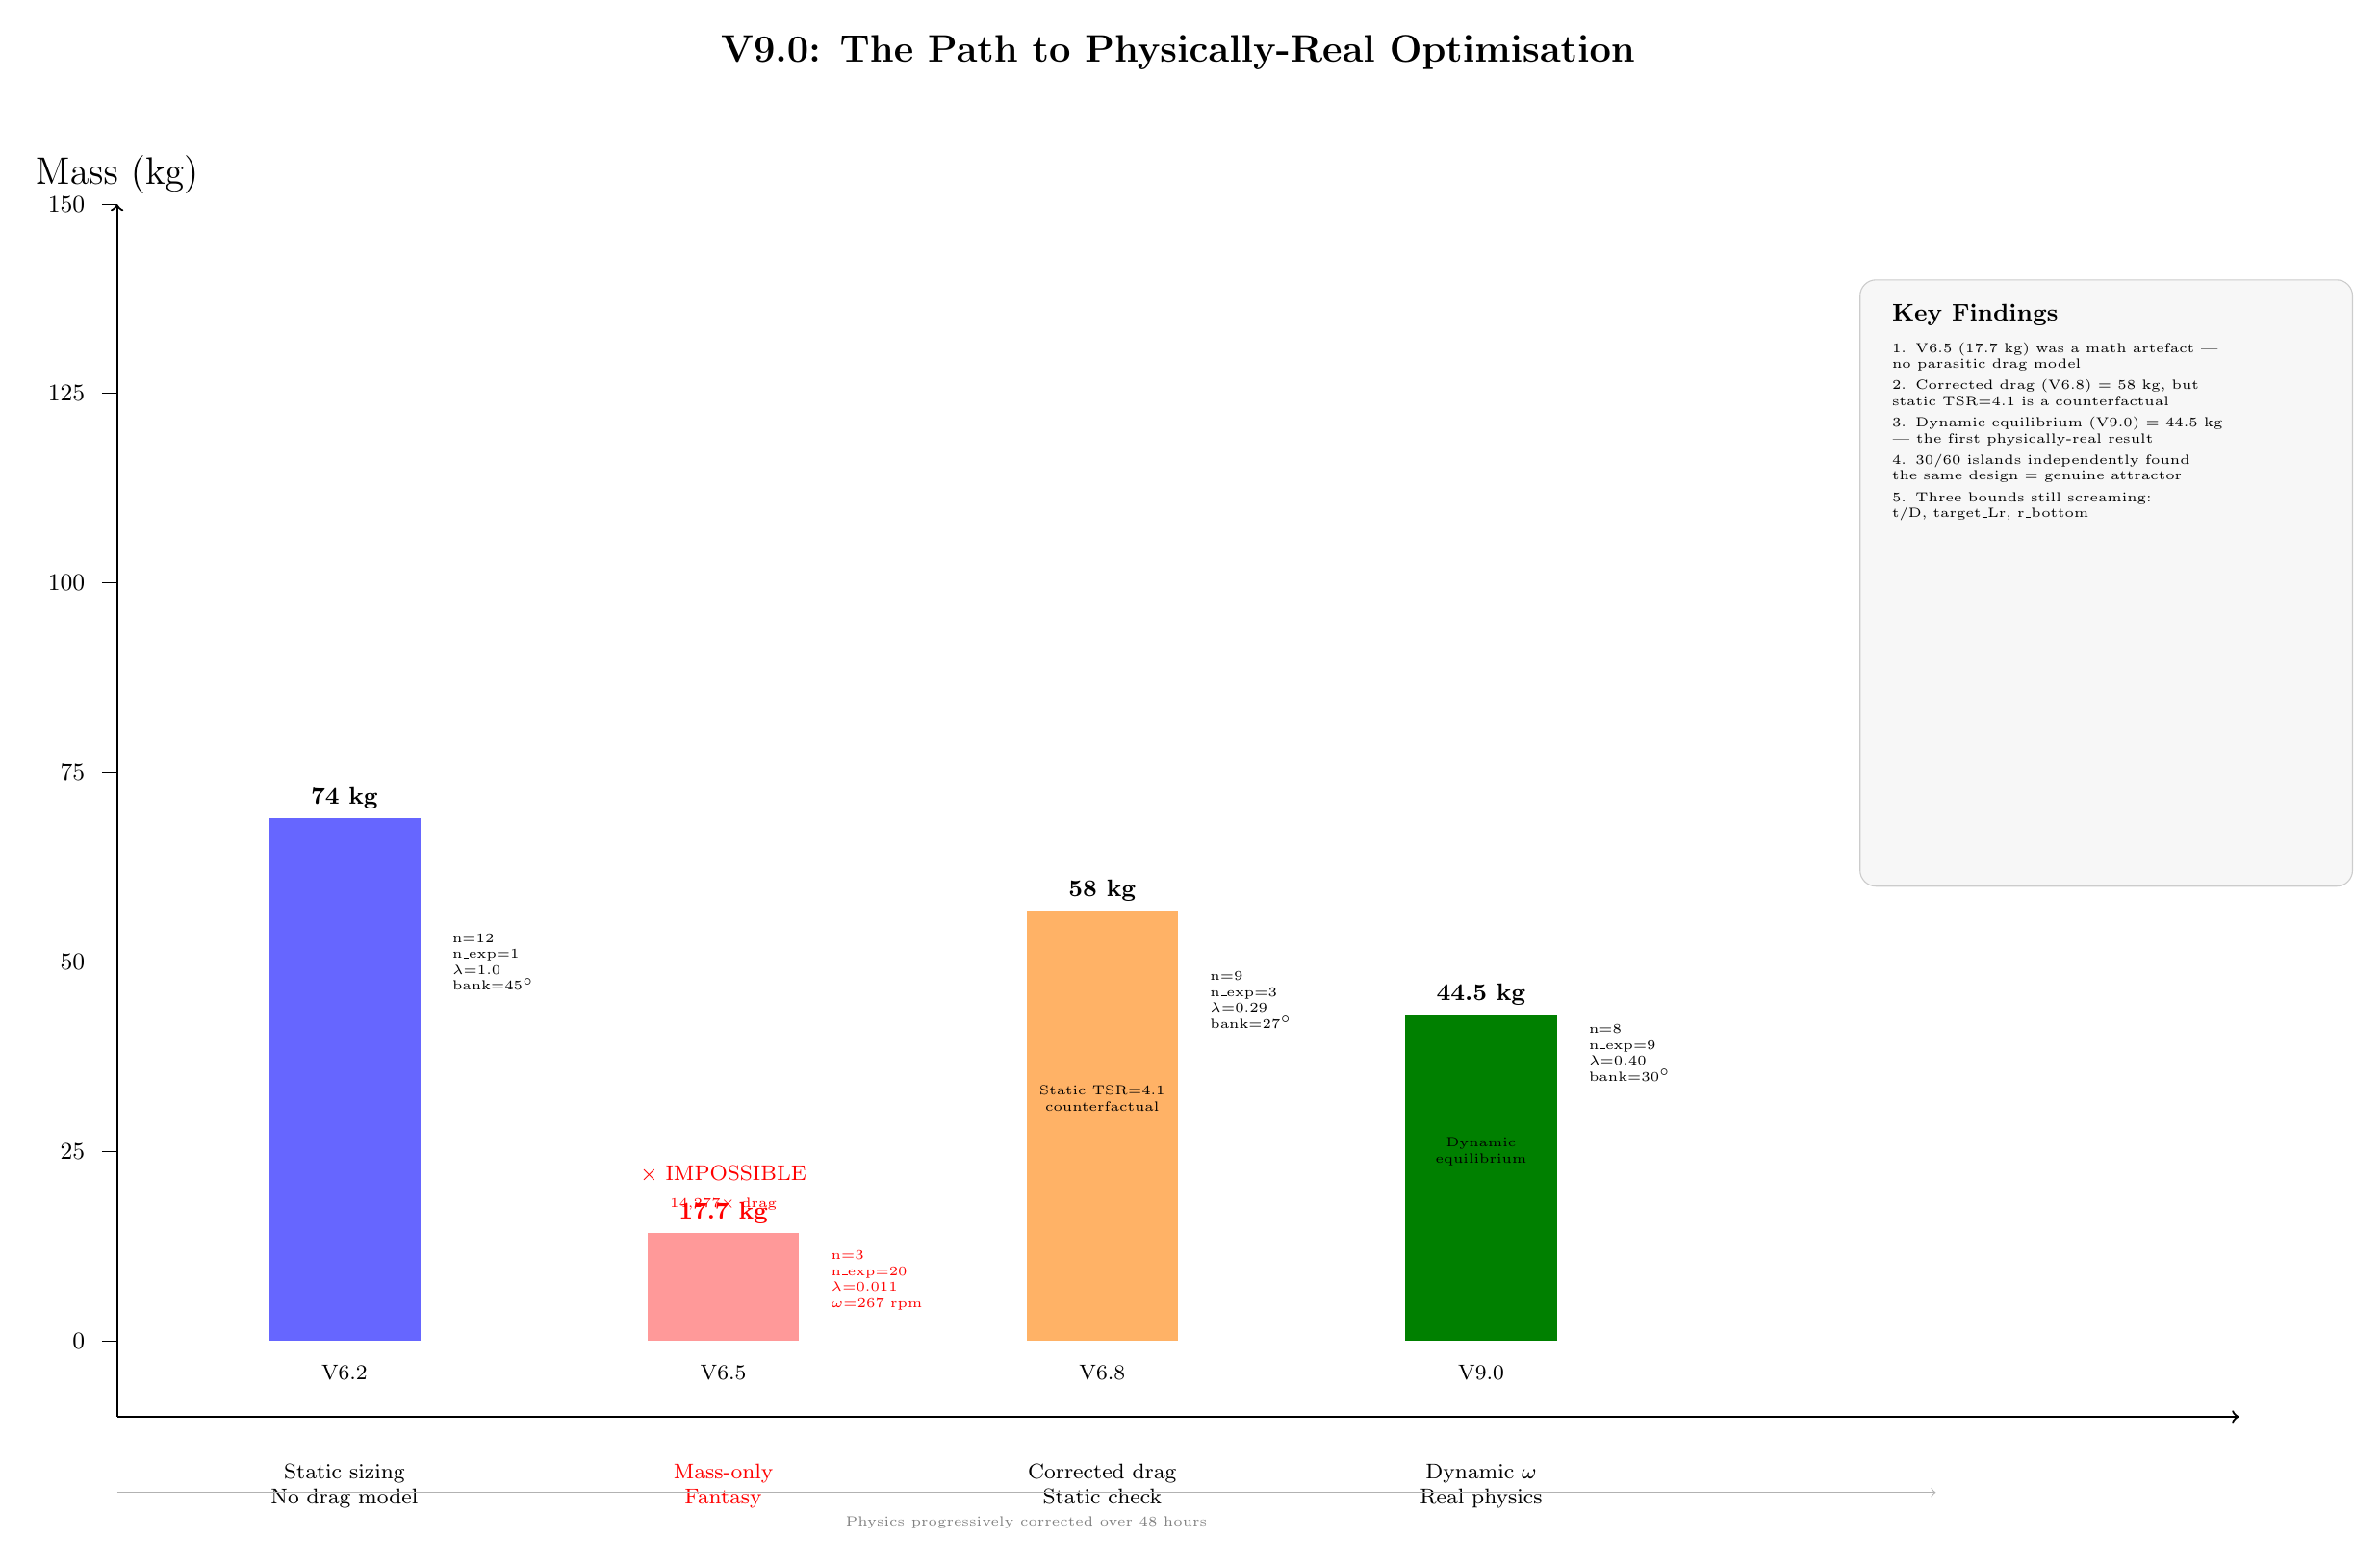
\begin{tikzpicture}[scale=1.0]

% ── Axes ──
\draw[->, thick] (1, 2) -- (1, 18) node[above] {\Large Mass (kg)};
\draw[->, thick] (1, 2) -- (29, 2) node[right] {};

% ── Y-axis ticks ──
\foreach \y/\label in {3/0, 5.5/25, 8/50, 10.5/75, 13/100, 15.5/125, 18/150} {
    \draw (0.8, \y) -- (1, \y);
    \node[left] at (0.7, \y) {\small\label};
}

% ── Versions as grouped bars ──
% V6.2 group at x=4
\fill[blue!60] (3, 3) rectangle (5, 9.9);  % 74.2 kg $\rightarrow$ 6.9 above base
\node[above, font=\small\bfseries] at (4, 9.9) {74 kg};
\node[below, font=\footnotesize] at (4, 2.8) {V6.2};

% V6.5 group at x=9 (marked as impossible)
\fill[red!40, dashed] (8, 3) rectangle (10, 4.42);  % 17.7 kg
\node[above, font=\small\bfseries, red] at (9, 4.42) {17.7 kg};
\node[below, font=\footnotesize] at (9, 2.8) {V6.5};
\node[red, font=\footnotesize] at (9, 5.2) {$\times$ IMPOSSIBLE};
\node[red, font=\tiny] at (9, 4.8) {14,277$\times$ drag};

% V6.8 group at x=14
\fill[orange!60] (13, 3) rectangle (15, 8.68);  % 58.4 kg $\rightarrow$ 5.68 above base
\node[above, font=\small\bfseries] at (14, 8.68) {58 kg};
\node[below, font=\footnotesize] at (14, 2.8) {V6.8};
\node[font=\tiny, text width=3cm, align=center] at (14, 6.2) {Static TSR=4.1\\counterfactual};

% V9.0 group at x=19
\fill[green!50!black] (18, 3) rectangle (20, 7.30);  % 44.5 kg $\rightarrow$ 4.30 above base
\node[above, font=\small\bfseries] at (19, 7.30) {44.5 kg};
\node[below, font=\footnotesize] at (19, 2.8) {V9.0};
\node[font=\tiny, text width=3cm, align=center] at (19, 5.5) {Dynamic\\equilibrium};

% ── Key parameter callouts ──
% V6.2
\node[font=\tiny, text width=2.5cm, align=left, anchor=west] at (5.3, 8) {n=12\\n\_exp=1\\$\lambda$=1.0\\bank=45$^\circ$};

% V6.5
\node[font=\tiny, text width=2.5cm, align=left, anchor=west, red] at (10.3, 3.8) {n=3\\n\_exp=20\\$\lambda$=0.011\\$\omega$=267 rpm};

% V6.8
\node[font=\tiny, text width=2.5cm, align=left, anchor=west] at (15.3, 7.5) {n=9\\n\_exp=3\\$\lambda$=0.29\\bank=27$^\circ$};

% V9.0
\node[font=\tiny, text width=2.5cm, align=left, anchor=west] at (20.3, 6.8) {n=8\\n\_exp=9\\$\lambda$=0.40\\bank=30$^\circ$};

% ── Strategy labels ──
\node[font=\footnotesize, text width=4cm, align=center, anchor=north] at (4, 1.5) {Static sizing\\No drag model};
\node[font=\footnotesize, text width=4cm, align=center, anchor=north, red] at (9, 1.5) {Mass-only\\Fantasy};
\node[font=\footnotesize, text width=4cm, align=center, anchor=north] at (14, 1.5) {Corrected drag\\Static check};
\node[font=\footnotesize, text width=4cm, align=center, anchor=north] at (19, 1.5) {Dynamic $\omega$\\Real physics};

% ── Physics corrections timeline ──
\draw[->, gray!60] (1, 1) -- (25, 1);
\node[font=\tiny, gray] at (13, 0.6) {Physics progressively corrected over 48 hours};

% ── Title ──
\node[font=\Large\bfseries] at (15, 20) {V9.0: The Path to Physically-Real Optimisation};

% ── Findings box ──
\fill[black!3, draw=gray!40, rounded corners=6pt] (24, 9) rectangle (30.5, 17);
\node[font=\small\bfseries, anchor=north west] at (24.3, 16.8) {Key Findings};
\node[font=\tiny, text width=5.8cm, align=left, anchor=north west] at (24.3, 16.3) {
1. V6.5 (17.7 kg) was a math artefact ---\\no parasitic drag model\\[2pt]
2. Corrected drag (V6.8) = 58 kg, but\\static TSR=4.1 is a counterfactual\\[2pt]
3. Dynamic equilibrium (V9.0) = 44.5 kg\\--- the first physically-real result\\[2pt]
4. 30/60 islands independently found\\the same design = genuine attractor\\[2pt]
5. Three bounds still screaming:\\t/D, target\_Lr, r\_bottom
};

\end{tikzpicture}
\end{document}
